%vorlesung 12 vom 29.11.2010
\chapter{Graphenalgorithmen}
\section{Einführung}
\subsection{Definitionen}
\begin{Def}[Graph]
  \hspace{\parindent}Ein \textit{Graph} $G=(V, E)$ ist eine Menge von \textit{Knoten} $V$ und \textit{Kanten} $E$. Knoten werden auch Ecken oder englisch \textit{vertices} (von vertex) genannt, Kanten nennt man im Englischen \textit{edges}. Es gilt $E \subseteq \binom{V}{2}$, das heißt Kanten sind ungeordnete Paare über $V$.
\end{Def}

\begin{Def}[gerichteter Graph]
  \hspace{\parindent}Ein \textit{gerichteter Graph} ist ein Graph, in dem die Kanten definiert sind als $E \subseteq V \times V$ (geordnete Paare).
\end{Def}

\begin{Bsp}[gerichteter Graph]
  \hspace{\parindent}$V = \{1, \ldots, 7\} \quad E = \{(1,2), (2,2), (1,3), \ldots \}$
  
  \begin{figure}[htb]
    \centering
    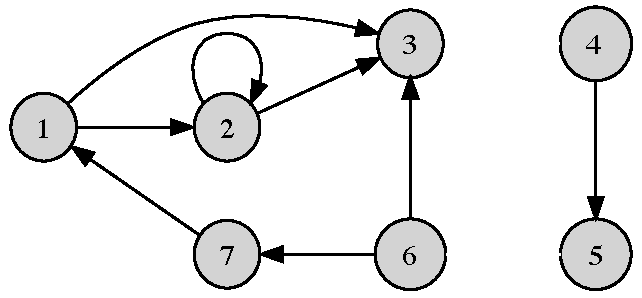
\includegraphics[scale=.5]{kap4Beispiel1}
    \caption{Ein gerichteter Graph}
    \label{kap4Beispiel1}
  \end{figure}
\end{Bsp}

\begin{Def}[Weg in einem Graphen]
  \hspace{\parindent}Ein \textit{Weg} in einem Graphen $G=(V,E)$ ist eine Folge von Knoten $v_1, \ldots, v_n$, wobei $(v_{i}, v_{i+1}) \in E$ für alle $i=1,\ldots n-1$. Die \textit{Länge eines Weges} ist $n-1$. Ein Weg $v_1, \ldots, v_n$ heißt \textit{einfach} genau dann, wenn $v_i \neq v_j$ für $i \neq j$ gilt.
\end{Def}

\begin{Def}[Kreis in einem Graph]
  \hspace{\parindent}Ein Weg $v_1, \ldots, v_n$ heißt \textit{Kreis} genau dann, wenn $v_1=v_n$. Ein Kreis heißt \textit{einfach}, wenn $v_i \neq v_{i+1}$ für alle $i=1, \ldots n-1$.
\end{Def}

\begin{Def}[azyklischer Graph]
  \hspace{\parindent}Ein Graph heißt \textit{azyklisch}, wenn er keinen Kreis enthält.
\end{Def}

\begin{Def}[zusammenhängender Graph]
  \hspace{\parindent}Ein ungerichteter Graph heißt \textit{zusammenhängend} genau dann, wenn zwischen je zwei Knoten $u,v \in V$ ein Weg $u=v_1, \ldots v_n = v$ existiert. Ein gerichteter Graph heißt \textit{stark zusammenhängend} genau dann, wenn zwischen je zwei Knoten $u,v \in V$ ein Weg $u=v_1, \ldots v_n = v$ existiert.
\end{Def}

\begin{Def}[Teilgraph]
  \hspace{\parindent}Ein Graph $G' = (V', E')$ heißt \textit{Teilgraph} eines Graphen $G=(V,E)$ genau dann, wenn $V' \subseteq V$ und $E' \subseteq E$. Ein Teilgraph heißt \textit{induzierter Teilgraph} genau dann, wenn $E' = E \bigcap (V' \times V')$ im gerichteten Fall und $E' = E \bigcap \binom{V'}{2}$ im ungerichteten Fall. Ein induzierter Teilgraph enthält also all die Kanten, die in $G$ zwischen den Knoten verlaufen, die auch in $V'$ enthalten sind.
\end{Def}

\begin{Def}[Zusammenhangskomponente]
  \hspace{\parindent}Eine \textit{Zusammenhangskomponente} von $G$ ist der maximale zusammenhängende induzierte Teilgraph $G' = (V', E')$. Maximal bedeutet, dass es keine echte Obermenge $V' \subsetneqq V''$ gibt, so dass der induzierte Teilgraph $G''=(V'', E'')$ zusammenhängend ist. Ist $G$ gerichtet, so spricht man von einer \textit{starken Zusammenhangskomponente}.
\end{Def}

\subsection{Darstellung endlicher Graphen}
Es gibt viele Möglichkeiten einen endlichen Graphen darzustellen, häufig genutzt werden die Adjazenzmatrix, die Adjazenzliste und die Inzidenzmatrix. Im folgenden gehen wir ohne Beschränkung der Allgemeinheit davon aus, dass der darzustellende Graph $G$ aus der Knotenmenge $\{ 1, \ldots, n \}$ besteht.

Eine \textit{Adjazenzmatrix} ist eine $n \times n$-Bitmatrix $A$. Für jeden Knoten enthält die Matrix eine Spalte und eine Zeile, dem entsprechend braucht eine Adjazenzmatrix $\Theta(n^2)$ Platz, mit $n = |V|$. $a_{ij} = 1 \Leftrightarrow (i,j) \in E$, die Matrix speichert also die zwischen Knoten verlaufenden Kanten. In ungerichteten Graphen gilt $a_{ij} = a_{ji}$.

\textit{Adjazenzlisten} speichern zu jedem Knoten $v$ eine Liste aller adjazenten Knoten, also alle $u$ mit $(v, u) \in E$. Adjazenzlisten brauchen $\Theta(n + m)$ viel Platz, mit $n = |V|$ und $m = |E|$.

Eine \textit{Inzidenzmatrix} hat für jeden Knoten eine Zeile und für jede Kante eine Spalte. Jede Spalte kann maximal zwei Einträge beinhalten, die sich von $0$ unterscheiden. Im ungerichteten Fall wird $1$ bei Knoten $v$ und Kante $e$ eingetragen genau dann, wenn $v$ inzident zu $e$ ist, das heißt wenn $v$ einer der beiden Endpunkte von $e$ ist. Im Fall eines azyklischen gerichteten Graphen wird beim Startknoten eine $1$ eingetragen und beim Endknoten eine $-1$.

\begin{Def}[Grad eines Knotens]
  \hspace{\parindent}Der \textit{Grad} eines Knotens entspricht im ungerichteten Fall der Anzahl inzidenter Kanten. Im gerichteten Fall wird zwischen dem \textit{Ingrad} und dem \textit{Ausgrad} unterschieden.
\end{Def}

\begin{Def}[Traversieren von Graphen]
  \hspace{\parindent}Als \textit{traversieren} von Graphen bezeichnet man das systematische besuchen aller Knoten eines Graphen, in dem man entlang der Kanten läuft. Hierzu gibt es zwei Techniken: Breiten- und Tiefensuche.
\end{Def}

Die \textit{Breitensuche} (BFS, \textit{breadth first search}) durchsucht $G=(V, E)$ bei $v$ beginnend. BFS findet alle direkten Nachbarn von $v$ und speichert sie in einer Warteschlange (Queue). Solange in der Warteschlange Knoten gespeicher sind, fügt es die noch nicht gefundenen Nachbarn des ersten Knotens der Warteschlange an die Warteschlange an. Dieser Vorgang wird solange wiederholt, bis die Warteschlange leer ist und keine unbekannten Knoten mehr gefunden werden. BFS findet kürzeste Wege in $G$, die von $v$ ausgehen. Die Laufzeit liegt in $\mathcal{O}(n^2)$, wenn $G$ als Adjazenzmatrix vorliegt und in $\mathcal{O}(n+m)$ bei der Darstellung von $G$ als Adjazenzliste.

Die \textit{Tiefensuche} (DFS, \textit{depth first search}) benutzt Rekursion oder einen Kellerspeicher (Stack). Alle Nachbarn eines Knotens $v$ werden darauf untersucht, ob sie bereits gefunden wurden. Die Knoten, die noch unbekannt sind werden in einen Speicher gelegt. Anschließend wird der oberste Knoten aus dem Kellerspeicher genommen und genauso untersucht. Dieses Verfahren wird angewandt, bis der Kellerspeicher leer und alle Knoten untersucht sind. Die Laufzeit liegt in $\mathcal{O}(n^2)$, wenn der zu untersuchende Graph als Adjazenzmatrix dargestellt wird, beziehungsweise in $\mathcal{O}(n+m)$ bei der Darstellung als Adjazenzliste. Die Tiefensuche findet alle Knoten zu denen es einen Weg von $v$ aus gibt (im ungerichteten Graphen ist das genau die Zusammenhangskomponente, die $v$ enthält).

Speichert man die Reihenfolge, in der die Knoten bei der Breiten- oder Tiefensuche entdeckt werden, kann man einen BFS-Baum beziehungsweise einen DFS-Baum aufstellen. Die Nummern der Reihenfolge (BFS- beziehungsweise DFS-Nummer) ist nicht eindeutig: Hat ein Knoten $v$ mehr als einen Nachbarn, wird bei BFS und DFS zufällig entschieden, welcher der Nachbarn zuerst besucht wird.

\begin{figure}[hbt]
  \centering
  \subfloat[\label{kap4BfsDfsBaum}]{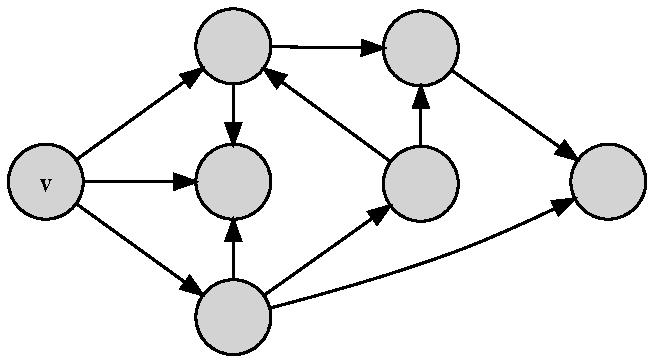
\includegraphics[width=.45\textwidth]{kap4BfsDfsBaum}}\\
  \subfloat[\label{kap4BfsBaum}]{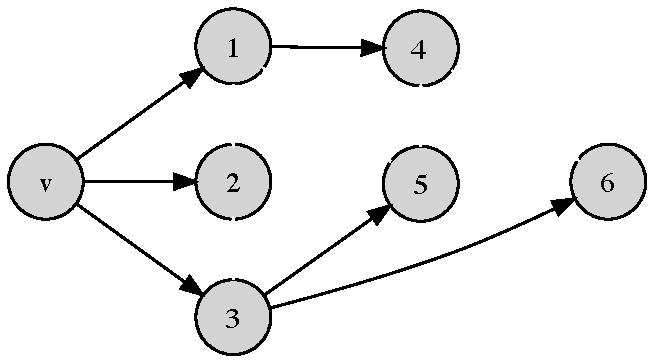
\includegraphics[width=.45\textwidth]{kap4BfsBaum}}\hspace{.05\textwidth}
  \subfloat[\label{kap4DfsBaum}]{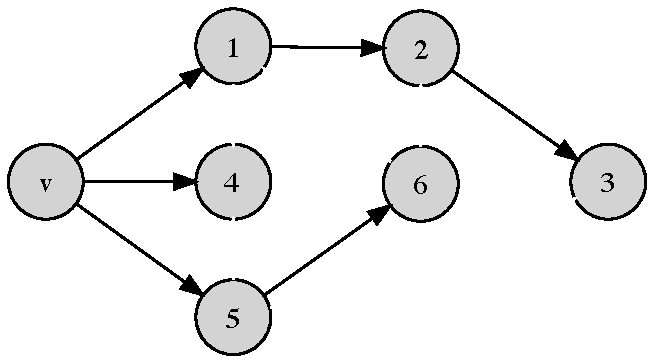
\includegraphics[width=.45\textwidth]{kap4DfsBaum}}
  \caption{\subref{kap4BfsDfsBaum} zeigt einen Graphen, \subref{kap4BfsBaum} einen zugehörigen BFS-Baum und \subref{kap4DfsBaum} einen zugehörigen DFS-Baum. In den DFS- und BFS-Baum sind die BFS- bzw. DFS-Nummern der Knoten eingetragen. BFS-Bäume enthalten kürzeste Wege vom Startknoten $v$ zu jedem anderen im Baum enthaltenen Knoten, so alle Kantenkosten identisch sind.}
  \label{kap4BfsDfsBaeume}
\end{figure}

\section{Minimale Spannbäume}
Gegeben ist ein ungerichteter Graph $G=(V,E)$ und eine Kostenfunktion $c: E \to \mathbb{R_+}$, die jeder Kante des Graphen Kosten zuweist. Gesucht ist ein zusammenhängender azyklischer Teilgraph $G'=(V, E')$ mit minimalen Gesamtkosten.

\begin{figure}[htb]
  \centering
  \subfloat[\label{kap4MST1}]{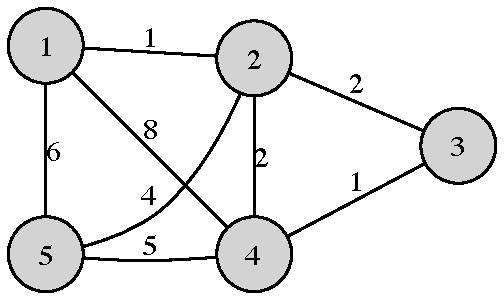
\includegraphics[width=.4\textwidth]{kap4MST1}}\hspace{.05\textwidth}
  \subfloat[\label{kap4MST2}]{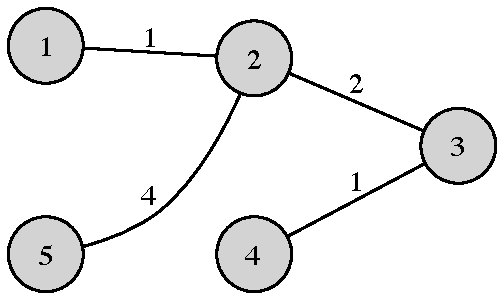
\includegraphics[width=.4\textwidth]{kap4MST2}}
  \caption{\subref{kap4MST2} ist ein minimaler Spannbaum des Graphen aus Abbildung \subref{kap4MST1}.}
  \label{kap4MST}
\end{figure}

\begin{Def}[Baum]
\hspace{\parindent}Ein \textit{Baum} ist ein azyklischer, zusammenhängender Graph.
\end{Def}

\begin{Def}[Spannbaum]
\hspace{\parindent}Ein \textit{Spannbaum} des Graphen $G=(V,E)$ ist ein Teilgraph $T=(V, E')$, der ein Baum (azyklisch, zusammenhängend) ist.
\end{Def}

Der \textit{Algorithmus von Kruskal} dient dem Finden von Spannbäumen minimaler Kosten. Er beginnt mit einem "`Spannwald"' $\{v_1\} \ldots \{v_n\}$.

\begin{Alg}[Algorithmus von Kruskal]
\begin{algorithmic}[1]
  \State $T := \emptyset$
  \State $Q := E$ \Comment{Prioritätswarteschlange gemäß Kosten}
  \State $VS := \{ \{v_1\} \ldots \{v_n\} \}$ \Comment{Partition der Knotenmenge}
  \While{$|VS| > 1$}
    \State $e:=\text{\texttt{delete-min}}(Q)$
    \If{$u, v$, mit $e=(u,v)$, liegen nicht in der gleichem Menge der Partion $VS$}
      \State Vereinige in $VS$ die Mengen, die $u$ und $v$  enthalten
      \State $T := T \cup \{ e \}$
    \EndIf
  \EndWhile
\end{algorithmic}
\end{Alg}

Als Datenstruktur für $Q$ bietet sich ein Heap an. Für $VS$ nutzen wir eine Union"=Find"=Struktur, mittels \texttt{Find} lässt sich leicht feststellen, ob $u$ und $v$ in der gleichen Menge der Partition liegen oder nicht, mit \texttt{Union} lassen sich bei Bedarf die Mengen, in denen $u$ und $v$ liegen leicht vereinigen. Die Initialisierung in Zeile $2$ liegt also in $\mathcal{O}(m \log m)$, die von Zeile $3$ in $\mathcal{O}(n)$. Die Laufzeit von Zeile 5 liegt in $\mathcal{O}(\log m)$ und wird $m$-mal ausgeführt, liegt insgesamt also in $\mathcal{O}(m \log m)$. Die Laufzeit der Zeilen 6 und 7 liegt insgesamt in $\mathcal{O}((n+m) \log^{*}n)$. Insgesamt liegt die Laufzeit des Algorithmus von Kruskal also in $\mathcal{O}(m \log m)$.

Der Algorithmus von Kruskal folgt einer einfachen Strategie, die als \textit{Greedy-Strategie} bekannt ist. Er sortiert alle Kanten nach ihren Kosten. Er betrachtet sich dann die jeweils günstigste noch nicht betrachtete Kante. Liegen die beiden Endknoten der Kante in unterschiedlichen Zusammenhangskomponenten, so fügt er die Kante zu seiner Lösung hinzu und vereinigt damit die beiden Zusammenhangskomponenten.

Der Algorithmus von Kruskal nimmt immer die nächste günstigste Kante. Die Strategie eines Algorithmus immer das nächste Beste zu bearbeiten nennt man \textit{greedy} (gierig). Auf abstrakte Strukturen verallgemeinernd können wir festhalten: greedy Algorithmen funktionieren auf \textit{Matroiden}.

%\section{Wegeprobleme in gerichteten Graphen}
%Gegeben sind ein gerichteter Graph $G=(V, E)$ und eine Kostenfunktion $c : E \to \mathbb{R}$. Häufig gestellte Fragen sind dann:
%
%\begin{enumerate}\renewcommand{\labelenumi}{\alph{enumi})}
%  \item Finde einen Weg mit minimalen Kosten, von $u$ nach $v$, mit $u,v \in V$.
%  \item Finde alle Wege mit minimalen Kosten von einem Knoten $u \in V$ zu jedem $v \in V$. Dieses Problem nennt man \textit{SSSP} (\textit{single source shortest path}).
%  \item Finde Wege mit minimalen Kosten zwischen allen Knotenpaaren $u, v$. Diese Fragestelltung wird \textit{APSP} (\textit{all pairs shortest path}) genannt.
%\end{enumerate}

%SSSP: Algorithmus von Daijkstra kurz erklären

%vorlesung 13 03.12.2010 (Fr)
%Ehe wir uns mit kürzesten"=Wege"=Problemen beschäftigen, sollten wir uns von der Korrektheit des Kruskal-Algorithmus überzeugen.

\subsection{Korrektheit des Kruskal"=Algorithmus (Greedy)}
Warum arbeitet der Algorithmus von Kruskal korrekt (beliebte Frage in Prüfungen)?

\begin{Lma}\label{kap4LmaKruskal}
\hspace{\parindent}Gegeben sind ein ungerichteter gewichteter Graph $G=(V, E)$ und ein aufspannender Wald $(V_1, T_1) \ldots (V_k, T_k)$ und $T=T_1 \cup \ldots \cup T_k$. Sei $e=(u,v)$ eine Kante mit minimalen Kosten und $u \in V_1$, $v \notin V_1$. Dann existiert der aufspannende Baum von $G$, der $T \cup \{e\}$ enthält und minimale Kosten unter allen Bäumen hat, die $T$ enthalten.
\end{Lma}

\begin{figure}[htb]
  \centering
  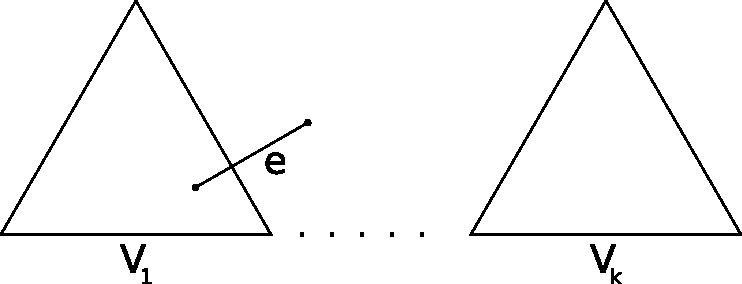
\includegraphics[scale=.5]{kap4KruskalErkl1}
  \caption{Die Ausgangslage des Lemmas \vref{kap4LmaKruskal}.}
  \label{KruskalErkl1}
\end{figure}

Aus Lemma \vref{kap4LmaKruskal} folgt die Korrektheit des Kruskal"=Algorithmus durch Induktion über seine Schleife.
Wir zeigen: jeder Wald, der bei Kruskals Algorithmus entsteht, ist Teilgraph eines minimal aufspannenden Baumes. Als Induktionsanfang dient uns bereits die Ausgangslage von Kruskals Algorithmus. Nach $0$ Iterationen besteht der Wald aus einem einzelnen Knoten.

Es folgt der Iterationsschritt von $k$ Iterationen auf $k+1$ Iterationen. Die Bäume $(V_1, T_1) \ldots (V_k, T_k)$ sind Teilgraphen eines minimal spannenden Baums (MST, \textit{minimum spanning tree}) nach Induktionsvoraussetzung. $e$ sei Kante minimalen Gewichts, die aus einem $V_i$ herausführt. Wenn man sie hinzu nimmt, dann gibt es nach Lemma \ref{kap4LmaKruskal} immer noch einen MST, der $T_1 \cup \ldots \cup T_k \cup \{e\}$ enthält. Es bleibt das Lemma zu Beweisen.

\begin{Bew}[Lemma \ref{kap4LmaKruskal}]
  \hspace{\parindent}Sei $B$ ein aufspannender Baum, der $T$ enthält und unter den Bäumen, die $T$ enthalten, minimale Kosten hat. Falls $e \in B$ ist das Lemma erfüllt. Andernfalls füge $e$ in $B$ ein. Es entsteht ein Kreis, denn $B$ enthält eine Kante $e' = (u', v')$ mit $u' \in V_1$, $v' \notin V_1$ und $e' \neq e$.  Es folgt $c(e) \le c(e')$ da $e$ minimal mit dieser Eigenschaft war.
  
  \begin{figure}[htb]
    \centering
    \includegraphics[scale=.32]{kap4BewKruskalLma}
    \caption{Wir sehen den Graphen $G$, sowie die Teilgraphen $V_1, \ldots, V_k$. $V_1$ ist ein aufspannender Baum, der $T$ enthält. Fügen wir nun eine Kante $e=(u,v)$ mit $u \in V_1$ und $v \notin V_1$ hinzu, gibt dies einen Kreis, da er bereits eine Kante $e'=(u', v')$ mit $u' \in V_1$ und $v \notin V_1$ enthält: Da $V_1$ ein Baum ist gibt es einen Weg von $u$ nach $u'$. Außerdem gibt es einen Weg von $v$ nach $v'$ (im Zweifelsfall über die Wurzel von $G$).}
  \end{figure}
  
  Wir schaffen nun einen neuen aufspannenden Baum $B'$, indem wir in $B$ $e'$ durch $e$ ersetzen. $B'$ enthält dann $T \cup \{e\}$. Es gilt $c(B') \le c(B)$, also ist $c(B')$ auch minimal unter Bäumen die $T$ enthalten (genau genommen gilt sogar $c(e) = c(e')$ und $c(B) = c(B')$).
\end{Bew}


\section{Wegeprobleme in gerichteten Graphen}
Gegeben ist im Allgemeinen ein gerichteter Graph $G=(V, E)$ mit Kostenfunktion $c : E \to \mathbb{R}$. Häufig gestellte Fragen sind dann:

\begin{itemize}\renewcommand{\labelenumi}{\alph{enumi})}
  \item Finde einen Weg mit minimalen Kosten, von $u$ nach $v$, mit $u,v \in V$.
  \item Finde Wege mit minimalen Kosten von einem Knoten $u \in V$ zu jedem anderen Knoten $v \in V$. Dieses Problem nennt man \textit{SSSP} (\textit{single source shortest path}).
  \item Finde Wege mit minimalen Kosten zwischen allen Knoten. Dieses Problem wird \textit{APSP} (\textit{all pairs shortest path}) genannt.
\end{itemize}

Wege mit minimalen Kosten werden manchmal auch \textit{kürzeste Wege} genannt. Als \textit{kürzesten Weg} kann man aber auch den Weg verstehen, der am wenigsten Kanten enthält. Im folgenden sprechen wir vom kürzesten Weg auch wenn wir den günstigsten Weg meinen. Aus dem Zusammenhang sollte eh hervorgehen, was gemeint ist (ein ungewichteter Graph entspricht einem gewichtetem Graph, bei dem alle Kantengewichte gleich sind).

\subsection{Dijkstras Algorithmus}
SSSP lässt sich mit Dijkstras Algorithmus lösen. Diesen Algorithmus wollen wir im folgenden vorstellen. Dabei bezeichnet $c[i,j]$ die Kosten der Kante $(i,j)$ falls $(i,j) \in E$. Es gilt $c[i,j] = \infty$ falls $(i,j) \notin E$. In $S$ speichern wir die Kontenmenge der Knoten zu denen bereits kürzeste Wege gefunden wurden. $D[v]$ bezeichnet die Kosten des kürzesten Weges von $s$ nach $v$.

\begin{Alg}[Dijkstra"=Algorithmus]
\begin{algorithmic}[1]
  \State $S :	= \emptyset$
  \State $D[s] := 0$
  \ForAll{$v \in V \setminus \{s\}$}
%    \State $D[v] := c[s,v]$
    \State $D[v] := \infty$
  \EndFor
  \While{$|S| < n$}
    \State wähle Knoten $w$ mit $w \in V \setminus S$ und $D[w]$ ist minimal
    \State $S := S \cup \{ w \}$
    \ForAll{$u \in V \setminus S$ und $u$ adjazent zu $w$}
      \State $D[u] := min(D[u], D[w] + c(w,u))$
    \EndFor
  \EndWhile
\end{algorithmic}
\end{Alg}

\subsubsection{Korrektheit von Dijsktra}
\begin{Beh}
  \hspace{\parindent}Zu jedem Zeitpunkt nachdem ein Knoten $w \in V$ in $S$ aufgenommen wird (Zeile 8) entspricht $D[w]$ genau der Länge des kürzesten Weges von $s$ nach $w$.
\end{Beh}

\begin{Bew}
  \hspace{\parindent}Der Beweis erfolgt per Induktion über die Anzahl $k$ der Iterationen der while-Schleife (Zeilen 6--12). Als Induktionsanfang wählen wir $k=0$. $S$ entspricht dann der leeren Menge, die Behauptung ist erfüllt. Wir können auch $k=1$ betrachten. Der Dijkstra"=Algorithmus wählt den Knoten $s$, es gibt keinen Knoten, der s näher sein kann, als s selbst. Der Abstand von s zu sich selbst entspricht $D[s] = 0$.
  
  Ehe wir den Induktionsschritt betrachten, führen wir noch $d(w)$ ein. $d(w)$ steht für die tatsächlichen Kosten des kürzesten Weges von $s$ nach $w$. In der $k$-ten Iteration der While"=Schleife werde $w$ aufgenommen. Wir nehmen an, dass wir den kürzesten Weg von $s$ nach $w$ noch nicht gefunden haben, das heißt $d(w) < D[w]$.
  
  \begin{figure}[htb]
    \centering
    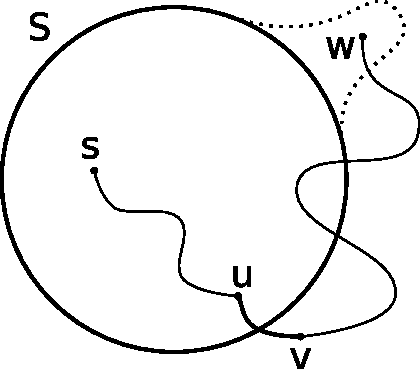
\includegraphics[scale=.66]{kap4DijkstraKorrekt}
    \caption{Betrachten den tatsächlich kürzesten Weg $\pi$ von $s$ nach $w$: $\pi$ verlässt die Menge $S_{k-1}$ zum ersten Mal beim Traversieren der Kante $(u, v)$.}
    \label{kap4DijkstraKorrekt}
  \end{figure}
  
  Betrachten wir den tatsächlich kürzesten Weg $\pi$ von $s$ nach $w$. $\pi$ verlässt die Menge $S_{k-1}$ zum ersten Mal beim Traversieren der Kante $(u,v)$. Das Stück von $\pi$ bis $u$ ist der kürzeste Weg von $s$ nach $u$. Nach Induktionsvoraussetzung ist seine Länge $d(u) = D[u]$.
  
  Es muss gelten $d(v) \le d(u) + c(u,v) = D[u] + c(u,v) \ge D[v]$, denn $D[v]$ wurde auf $min(D[v], D[u] + c(u,v))$ gesetzt als $u$ in $S$ aufgenommen wurde. Tatsächlich gilt $D[v] = d(v)$, denn $d(u) + c(u,v)$ ist Teil des tatsächlich kürzesten Wegs $\pi$ von $s$ nach $w$. Des Weiteren muss gelten $D[w] \ge d(w) > d(v) = D[v]$. Dass steht aber im Widerspruch zum Dijkstra"=Algorithmus, der in Zeile 7 $w$ danach ausgesucht hat, dass $D[w]$ minimal ist.
  
  Somit haben wir bewiesen: zu jedem Zeitpunkt nachdem Knoten $w \in V$ in $S$ aufgenommen wird (Zeile 8) ist $D[w]$ die Länge des kürzesten Weges von $s$ nach $w$. Der Dijkstra"=Algorithmus arbeitet also korrekt.
\end{Bew}

\subsubsection{Laufzeit des Dijkstra"=Algorithmus}
Um eine Aussage über die Laufzeit des Dijkstra"=Algorithmus treffen zu können, müssen wir uns kurz überlegen, welche Datenstrukturen wir nutzen. Für die Knoten in $V \setminus S$ nutzen wir eine Prioritätswarteschlange (Heap) gemäß des Wertes $D$, alle anderen Datenstrukturen sollten trivial sein. Die Laufzeit für die Initialisierung (Zeilen 2--5) liegt in $\mathcal{O}(n)$. Zeile 7 und 8 entsprechen einem Aufruf von \texttt{delete"=min}, liegen also in $\mathcal{O}(\log n)$. Sie werden $n$ mal aufgerufen, was insgesamt in $\mathcal{O}(n \log n)$ liegt. Zeile 10 entspricht einem Aufruf von \texttt{decrease"=key} und liegt somit in $\mathcal{O}(\log n)$. Sie wird höchstens einmal pro Kante ausgeführt, was insgesamt in $\mathcal{O}(m \log n)$ liegt. Die Laufzeit des gesamten Algorithmus liegt also in $\mathcal{O}((n+m)\log n)$.

\subsection{All Pairs Shortest Path (APSP)}
Möchte man die kürzesten Wege zwischen allen Knoten berechnen, so könnte man einfach den Dijkstra"=Algorithmus auf alle Knoten anwenden. Von der Laufzeit her ist das aber nicht besonders gut, es läge in $\mathcal{O}(n (n+m) \log n)$, was sich mit $\mathcal{O}(n^3 \log n)$ abschätzen lässt. Geht das schneller?

%Algorithmus von Floyd"=Warshall
%
%$G(V,E)$
%$V=\{1, \ldots, n\}$
%$c(i,j)= Kosten von (i,j) fall (i,j) \in E, \infty sonst$.
%
%berechnen Werte
%$d_{ij}^k$ $\Big\{$ \begin{tabular}{l}$1\le i,j \le n$ \\ $0 \le k \le n$\end{tabular}
%
%= Länge des kürzesten Weges von $i$ nach $j$ mit Zwischenkonten in $\{1, \ldots k\}$ $\infty$ falls kein solcher Weg existiert.
%
%$d_{ij}^0 = c(i, j)$
%
%$d_{ij}^k$ Zeichnung 13-4
%erste Möglichkeit $k$ kommt nicht vor auf kürzestem Weg von $i$ nach $j$ mit Zwischenknoten $\in \{1, \ldots, k\}$: $d_{ij}^k = d_{ij}^{k-1}$
%
%$d_{ij}^k := min(d_{ij}^{k-1}, d_{ik}^{k-1}, d_{kj}^{k-1})$
%2. Möglichkeit $k$ kommt vor (ohne weitere Einschränkung nur einmal) Zeichnung 13-4b dann $d_{ij}^k = d_{ik}^{k-1} + d_{kj}^{k-1}$

% vorlesung 14 vom 06.12.2010 (Mo)
%APSP

Sei $G=(V,E)$ ein gerichteter Graph mit Kostenfunktion $c: E \to \mathbb{R}_{\ge 0}$. Die Knotenmenge $V$ sei o.B.d.A. $\{1, \ldots, n\}$. $d_{ij}^{k}$ entspricht den Kosten des kürzesten Weges zwischen $i$ und $j$ mit Zwischenknoten $\in \{1, \ldots, k\}$. $d_{ij}^k$ ist entweder $d_{ij}^{k-1}$ oder $d_{ik}^{k-1} + d_{kj}^{k-1}$. Ein Algorithmus, der die Kosten aller kürzesten Wege unter Nutzung der Methode des dynamischen Programmierens berechnet, ist dann einfach zu finden.

\begin{Alg}[von Floyd"=Warshall (dynamisches Programmieren)]
  \begin{algorithmic}[1]
    \For{$i=1 \ldots n$}
      \For{$j=1 \ldots n$}
        \If{$(i,j) \in E$}
          \State $d_{ij}^0 = c(i,j)$
        \Else
          \State $d_{ij}^0 = \infty$
        \EndIf
      \EndFor
    \EndFor
    \For{$k=1 \ldots n$}
      \For{$i=1 \ldots n$}
        \For{$j=1 \ldots n$}
          \State $d_{ij}^k = min(d_{ij}^{k-1}, d_{ik}^{k-1} + d_{kj}^{k-1})$\label{kap6FWAlgEntfernungBerechnen}
        \EndFor
      \EndFor
    \EndFor
  \end{algorithmic}
\end{Alg}

%Algorithmus von Floyd"=Warshall (dynamisches Programmieren)
%
%for $i=1, \ldots, n$ do\\
%  for $j=1, \ldots, n$ do\\
%    $d_{ij}^0$ = $c(i,j)$ falls $(i,j) \in E$, $\infty$ sonst\\
%  done\\
%done\\
%for $k=1, \ldots, n$ do\\
%  for $i=1, \ldots n$ do\\
%    for $j=1, \ldots, n$ do\\
%      $d_{ij}^k = min (d_{ij}^{k-1}, d_{ik}^{k-1} + d_{kj}^{k-1})$\\
%    done\\
%  done\\
%done\\

Die Länge der tatsächlich kürzesten Wege finden wir dann in $d_{ij}^n$ mit $1 \le i, j \le n$. Die Laufzeit liegt aufgrund der dreifach verschachtelten Schleife in $\mathcal{O}(n^3)$. Für mehrfaches Ausführen des Dijkstra"=Algorithmus hatten wir eine Laufzeit von $\mathcal{O}(n (n+m) \log n)$ angegeben. Die Anzahl der Kanten $m$ kann maximal $n^2$ groß werden. In einem vollständigen Graphen hat das dann eine Laufzeit von $\mathcal{O}(n^3 \log n)$, hier ist also der Algorithmus von Floyd"=Warshall günstiger. Für dünn besetzte Graphen (mit maximal $\frac{n^2}{n \log n}$ Kanten) ist das mehrfache Ausführen des Dijkstra"=Algorithmus jedoch besser.

Tatsächlich lassen sich mit beiden Algorithmen nicht nur die Länge der kürzesten Wege bestimmen, sondern auch die Wege selber (Teil der Übung). Der Algorithmus von Floyd"=Warshall ist vielseitig anwendbar. Setzt man in der Initialisierung $c(i,j) = 0$ falls $(i,j) \notin E$ und $1$ andernfalls und ersetzt die die Operanden $min, +$ durch $\vee$ und $\wedge$, so berechnet der Algorithmus, ob es überhaupt einen Weg zwischen zwei Knoten gibt, er berechnet also den transitiven Abschluss des Graphen $G$.

Der Algorithmus von Floyd"=Warshall geht ursprünglich auf einen Algorithmus von Kleene zurück. Eigentlich ist der Algorithmus von Floyd"=Warshall eine Abwandlung des Algorithmus von Kleene, wir beschreiben den Algorithmus von Kleene hier dennoch wie eine Abwandlung des Floyd"=Warshall"=Algorithmus.

Der Algorithmus bekommt als Eingabe einen endlichen Automaten (DFA) und gibt den regulären Ausdruck aus, der der Sprache entspricht, die der DFA erkennt. Die Zustände des Automaten werden dabei als Knoten angesehen und die Kostenfunktion als Abbildung von Kanten auf Elemente des Alphabets, also $c: E \to \Sigma$. $d_{ij}^k$ entspricht der Menge von Wörtern, die der Automat erzeugen kann, wenn er in Zustand $i$ beginnt, in Zustand $j$ endet und nur die Zustände $1, \ldots, k$ nutzt. Dazu wird die Initialisierung geändert zu:
\[ d_{i,j}^0 = \begin{cases}
                 a^* & \text{falls $i=j$ und der DFA erzeugt $a$ auf dem Weg von $i$ nach $i$}\\
                 \{ \varepsilon \} & \text{falls $i=j$ und } (i,i) \notin E\\
                 b & \text{falls $i \neq j$ und } (i,j) \in E \\
                 \emptyset & \text{sonst}
\end{cases} \]
und Zeile \ref{kap6FWAlgEntfernungBerechnen} des oben angegebenen Algorithmus von Floyd"=Warshall wird ersetzt durch
\[ d_{ij}^k = d_{ij}^{k-1} \cup d_{ik}^{k-1} (d_{kk}^{k-1})^* d_{kj}^{k-1} \]

\section{Flüsse in Netzen (network flow)}
Sei ein gerichteter Graph $G=(V,E)$ gegeben mit Kapazitätsfunktion $c: E \to \mathbb{R}_{\ge 0}$, \textit{Quelle} $s \in V$ und \textit{Ziel} (auch \textit{Senke} genannt) $t \in V$. Ein Beispiel eines solchen Graphen sehen wir in Abbildung \vref{kap4Fluesse1}. Gesucht wird der \textit{maximale Fluss} von $s$ nach $t$.

\begin{Def}[Netz]
  \hspace{\parindent}Wir definieren ein \textit{Netz} (oder auch \textit{Netzwerk}) $(V, E, c, s, t)$ als einen gerichteten Graphen mit Kapazitätsfunktion $c: E \to \mathbb{R}_{\ge 0}$, Quelle $s \in V$ und Senke $t \in V$.
\end{Def}

\begin{figure}[htb]
  \centering
  \includegraphics[scale=.75]{kap4Fluesse1}
  \caption{Ein Graph mit Quelle $s$ und Senkte $t$ und Kapazitäten an den Kanten.}
  \label{kap4Fluesse1}
\end{figure}

In der Praxis gibt es einige Beispiele: Röhrensysteme für Öl, Gas, Wasser oder ähnliches, Evakuierungspläne, Verkehrsnetze und so weiter.

\begin{Def}[Fluss]
\hspace{\parindent}Ein \textit{Fluss} ist eine Funktion $f: V \times V \to \mathbb{R}$ mit folgenden Eigenschaften:
\begin{alignat*}{2}
  f(u,v) & \le c(u,v) &\qquad& \text{wobei } c(u,v) := 0 \text{ falls } (u,v) \notin E\\
  f(u,v) & = -f(v,u) \\
  \sum_{v \in V} f(u,v) & = 0 && \forall u \in V \setminus \{s,t\}
\end{alignat*}
\end{Def}

\begin{Def}[Wert eines Flusses]
  \hspace{\parindent}Den \textit{Wert eines Flusses} definieren wir als
  \[|f| := \sum_{v \in V} f(s,v)\]
\end{Def}

\begin{figure}[htb]
  \centering
  \includegraphics[scale=.75]{kap4Fluesse2}
  \caption{In dem Beispiel aus Abbildung \vref{kap4Fluesse1} wurde mittels einer Greedy-Strategie ein maximaler Fluss bestimmt. Die Zahlen entlang der Kanten geben zuerst die durch den Fluss genutzte Kapazität dann die verfügbare Kapazität an. Der Fluss hat eine Größe von $|f| = 23$.}
  \label{kap4Fluesse2}
\end{figure}

Hat man ein Netzwerk mit mehr als einer Quelle und einer Senke, kann man das leicht auf eine Netzwerk mit einer Quelle und einer Senke zurückführen. Abbildung \vref{kap4MultQuellenSenken} zeigt wie das geht.

\begin{figure}[htb]
  \centering
  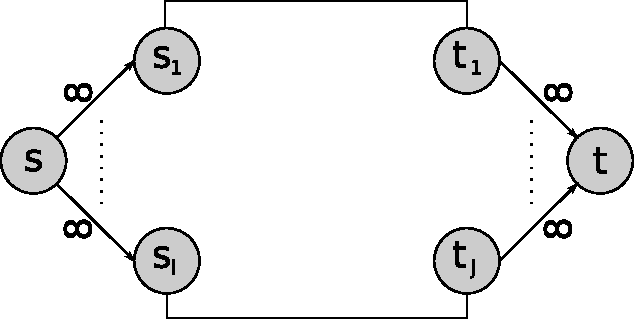
\includegraphics[scale=.75]{kap4MultQuellenSenken}
  \caption{Um ein Netzwerk mit mehr als einer Quelle und Senke zu einem Netzwerk mit einer Quelle und Senke zu wandeln führt man einen zusätzlichen Knoten $s$ und einen zusätzlichen Knoten $t$ ein. Von $s$ aus werden Kanten mit unendlich hoher Kapazität zu allen Quellen geführt und von den bestehenden Senken ebensolche Kanten zum Knoten $t$. $s$ wird dann Superquelle und $t$ Supersenke genannt.}
  \label{kap4MultQuellenSenken}
\end{figure}

\subsection{Ford"=Fulkerson"=Methode zur Bestimmung des maximalen Flusses}
Wie oben geschrieben suchen wir nach dem maximalen Fluss in einem solchen Netzwerk. Eine Methode dazu stammt von Ford und Fulkerson. Dazu wird im Netzwerk nach augmentierenden Wegen gesucht.

\begin{Def}[Augmentierender Weg]
  \hspace{\parindent} Gegeben ist ein Netzwerk mit einem Fluss $f$. Darin gibt es einen Weg von $s$ nach $t$, wobei für alle Kanten $(u,v)$ auf dem Weg gilt $f(u,v) < c(u,v)$. Das heißt alle Kanten auf dem Weg haben größere Kapazitäten, als sie bislang vom Fluss genutzt werden. Einen solchen Weg nennt man \textit{augmentierend}.
\end{Def}

\strut\begin{Alg}[Ford-Fulkerson]
  \begin{algorithmic}[1]
    \State initialisiere $f$ mit $0$ (auf jeder Kante).
    \While{augmentierender Weg exisitert}
      \State erhöhe den Fluss entlang dieses Weges so stark wie möglich.
    \EndWhile
  \end{algorithmic}
\end{Alg}

Beim Ausführen des Algorithmus von Ford"=Fulkerson hilft eine Datenstruktur, die wir Restnetz nennen.
\begin{Def}[Restnetz]
  \hspace{\parindent}Sei $G=(V,E)$ ein Graph mit Kapazitätsfunktion $c$, mindestens zwei Knoten $s$ und $t$ die als Quelle und Senke dienen und einem Fluss $f$. Das \textit{Restnetz} $G_f$ ist ein Graph mit der Knotenmenge $V$ und folgenden Kanten. Sei $e=(u, v) \in E$ eine Kante aus $G$ mit Kapazität $c(e)=b$, von der der Fluss bereits $f(e)=a$ nutzt. Dann hat die Kantenmenge des Restnetzes $E_f$ zwei Kanten: $(u,v)$ und $(v,u)$. Die Kapazitäten bestimmen wir wie folgt:
  \[ c_f(u,v) = b-a \]
  \[ c_f(v,u) = a \]
  
  Ist $c(u,v) = f(u,v)$ und somit $b-a = 0$, kann die Kante $(u,v)$ im Restnetz auch weggelassen werden. Analog kann auch die Kante $(v,u)$ weggelassen werden, wenn $f(u,v)=0$, also $b-a = b$.
\end{Def}

\begin{figure}[htb]
  \centering
  \subfloat[Eine einfache Kante im Netzwerk (links) wird ersetzt durch zwei Kante im Restnetz (rechts).\label{kap4RestnetzKonstruktion1}]{
    
\includegraphics[width=.25\textwidth]{kap4RestnetzKonstruktionA1}\hspace{4em}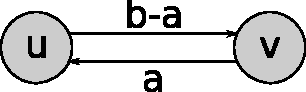
\includegraphics[width=.25\textwidth]{kap4RestnetzKonstruktionB1}}\\
  \subfloat[Bestehen im Netzwerk bereits zwei Kanten, so wird $a$ zur Rückwärtskante addiert.\label{kap4RestnetzKonstruktion2}]{
    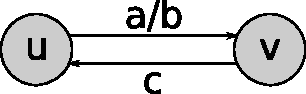
\includegraphics[width=.25\textwidth]{kap4RestnetzKonstruktionA2}\hspace{4em}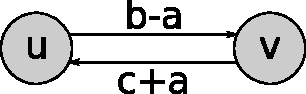
\includegraphics[width=.25\textwidth]{kap4RestnetzKonstruktionB2}}
  \caption{Zu sehen ist, wie Kanten des Netzwerkes bei der Konstruktion des Restnetzes ersetzt werden. $b$ bezeichnet die Kapazität einer Kante, $a$ die durch den Fluss genutzte Kapazität, $c$ die Kapazität einer im Netzwerk bestehenden Rückwärtskante.}
  \label{kap4RestnetzKonstruktion}
\end{figure}

Die Konstruktion der Kanten im Restnetz zeigt Abbildung \vref{kap4RestnetzKonstruktion}. Einen Fluss in unserem Beispielnetzwerk und das resultierende Restnetz zeigt Abbildung \vref{kap4FluesseRestnetz}.

\begin{figure}[htb]
  \centering
  \subfloat[\label{kap4Fluesse3}]{\includegraphics[width=.45\textwidth]{kap4Fluesse3}}\hspace{.025\textwidth}
  \subfloat[\label{kap4Fluesse4}]{\includegraphics[width=.45\textwidth]{kap4Fluesse4}}
  \caption{\subref{kap4Fluesse3} zeigt einen Fluss in unserem Beispielnetz. \subref{kap4Fluesse4} zeigt das resultierende Restnetz.}
  \label{kap4FluesseRestnetz}
\end{figure}

Ein augmentierender Weg in $G$ entspricht einem Weg von $s$ nach $t$ im Restnetz $G_f$. Der Ford"=Fulkerson"=Algorithmus kann somit vereinfacht werden:

\begin{Alg}[Ford"=Fulkerson mit Hilfsstruktur $G_f$]
  \begin{algorithmic}[1]
    \State $G_f := G$
    \While{finde Weg von $s$ nach $t$ in $G_f$}
      \State erhöhe Fluss entlang dieses Weges so weit wie möglich
      \State aktualisiere $G_f$
    \EndWhile
  \end{algorithmic}
\end{Alg}

Sind alle Kapazitäten im Netzwerk ganzzahlig, so sind es auch alle Kapazitäten im Restnetzwerk, da wir nur ganze Zahlen addieren und subtrahieren. Der Fluss wird dann in jeder Iteration des Algorithmus um mindestens $1$ erhöht, was wichtig für die Analyse der Laufzeit ist. Warum können wir o.B.d.A. annehmen, dass alle Kapazitäten ganzzahlig sind? Weil wir andernfalls alle Kapazitäten entsprechend erweitern könnten. Arbeiten wir nicht mit ausschließlich ganzzahligen Kapazitäten, kann es passieren, dass der Algorithmus nicht terminiert!

Betrachten wird die Laufzeit dieses Algorithmus. Dabei sei $|V| = n$ und $|E| = m$. Das Finden eines augmentierenden Weges entspricht dem Finden eines Weges von $s$ nach $t$ in $G_f$. Dies ist zum Beispiel durch Breiten- oder Tiefensuche in $\mathcal{O}(n+m)$ möglich. Wir können wie gesagt von ganzzahligen Kapazitäten und somit von einer Steigerung des Flusses je Iteration um mindestens $1$ ausgehen. Daraus folgt das maximal $|f^*|$ Iterationen nötig sind. Dabei ist $f^*$ der endgültige (maximale) Fluss. Die Laufzeit liegt also in $\mathcal{O}(|f^*| \cdot (m+n))$. $f^*$ kann exponentiell in der Eingabegröße sein, wenn die Kapazitäten als Binärzahlen gegeben sind. Ist eine Zahl in Binärdarstellung gegeben, so ist ihr Wert exponentiell ihrer Länge.

%vorlesung 15 2010-12-10 (Fr)

\begin{figure}[htb]
  \centering
  \includegraphics[scale=.66]{kap4FFWorstCase}
  \caption{Ein Netzwerk, in dem der Algorithmus von Ford"=Fulkerson unter Umständen eine schlechte Laufzeit aufweist (Beispiel für eine worst-case-Analyse).}
  \label{kap4FFWorstCase}
\end{figure}

%Bei jeder Augmentierung erhöht sich der Fluss um mindestens $1$. Insgesamt hat man also maximal $|f^*|$ Augmentierungen, wobei $|f^*|$ dem endgültigen (maximalen) Fluss entspricht. Eine Augmentierung benötigt $\mathcal{O}(n+m)$ Zeit mit zum Beispiel Tiefen- oder Breitensuche, insgesamt liegt der Algorithmus also in $\mathcal{O}(|f^*| \cdot (m+n))$. Das ist potentiell exponentiell in der Größe der Eingabe (ist eine Zahl in Binärdarstellung gegeben, so ist ihr Wert exponentiell ihrer Länge, hier geht es um die Form der Kapazitäten).

Abbildung \vref{kap4FFWorstCase} zeigt ein Netz, in dem es passieren kann, dass der Ford"=Fulkerson"=Algorithmus den Fluss um je $1$ erhöht, also $2000$ Augmentierungen braucht. Es ist klar, dass wir den Algorithmus entsprechend verbessern sollten, wie genau zeigen wir später.

\subsection{Schnitte}
\begin{Def}[Fluss zwischen zwei Knotenmengen]
  \hspace{\parindent}In einem Netzwerk $N=(V, E, c, s, t)$ seien $X, Y$ zwei Mengen von Knoten. Dann definieren wir den Fluss von $X$ nach $Y$ als
\[ f(X,Y) := \sum_{x \in X} \sum_{y \in Y} f(x,y) \]
\end{Def}

Durch nachrechnen liese sich leicht beweisen, dass bei Flüssen zwischen Knotenmengen folgendes gilt:
\begin{Lma}\label{Lemma41}
  \begin{alignat*}{2}
    f(X,X) &= 0 &\quad& \forall X \subset V\\
    f(X,Y) &= -f(Y,X) && \forall X,Y \subset V\\
    f(X \cup Y, Z) &= f(X,Z) + f(Y,Z) && \forall X,Y \subset V, X \cap Y = \emptyset\\
    f(Z, X \cup Y) &= f(Z,X) + f(Z,Y) && \forall X,Y \subset V, X \cap Y = \emptyset
  \end{alignat*}
\end{Lma}

\begin{Def}[Schnitt]
  \hspace{\parindent}Wir definieren den \textit{Schnitt eines Netzwerks} als eine Partition der Knotenmenge $V = S \cupdot T$ mit Quelle $s \in S$ und Senke $t \in T$. Es handelt sich also um zwei disjunkte Teilmengen, das heißt $S \cap T = \emptyset$.
\end{Def}

\begin{figure}[htb]
  \centering
  \includegraphics[scale=.75]{kap4DefSchnitt}
  \caption{Die Abbildung skizziert eine einfache Vorstellung eines Schnitts.}
  \label{kap4DefSchnitt}
\end{figure}

Den Fluss zwischen zwei Knotenmengen haben wir bereits definiert. Analog dazu definieren wir die Kapazität eines Schnitts:
\[c(S,T) = \sum_{x \in S} \sum_{y \in T} c(x,y)\]
und den Fluss eines Schnitts:
\[ f(S,T) = \sum_{x \in S} \sum_{y \in T} f(x,y) \]

\begin{Lma}\label{Lemma42}
  Für jeden Fluss $f$ und jeden Schnitt $S, T$ gilt: \[ f(S,T) = |f| \]
\end{Lma}

\begin{Bew}
  \begin{alignat*}{2}
    f(S,T) &= f(S, V) - f(S,S) &\quad& \text{ weil } f(S,V) = f(S,T) + f(S,S)\\
           &= f(S, V) && \text{ weil } f(S,S) = 0\\
           &= f(\{s\}, V) + f(S \setminus \{s\}, V)\\
%           &= |f| + \sum_{u\in S \setminus \{s\}} \sum_{v\in V} f(u,v)\\
           & = |f| && \text{ weil } f(S \setminus \{s\}, V) = 0 \text{ und } f(\{s\}, V) = |f|
  \end{alignat*}
\end{Bew}

\begin{Koro}
  \hspace{\parindent}Der Wert jedes Flusses $f$ ist nach oben beschränkt durch die Kapazität jedes beliebigen Schnittes $S, T$:
  \[ |f| \le c(S,T) \]
  Dies gilt für jeden Fluss $f$ und jeden Schnitt $S$, also auch für den maximalen Fluss und den minimalen Schnitt.
\end{Koro}

\begin{Satz}[maximaler Fluss - minimaler Schnitt]
  \hspace{\parindent}Sei $f$ ein Fluss in einem Netzwerk $(V, E, c, s, t)$. Sei $G_f$ das entsprechende Restnetzwerk. Dann sind folgende Aussagen äquivalent:
  \begin{enumerate}
    \item \label{kap4SatzMaxFMinS:fMax} $f$ ist maximal.
    \item \label{kap4SatzMaxFMinS:augWeg} Es gibt keine augmentierenden Wege.
    \item \label{kap4SatzMaxFMinS:minS} Es gibt einen Schnitt $S,T$ mit $|f| = c(S,T)$.
  \end{enumerate}
\end{Satz}

\begin{Bew}
  \hspace{\parindent}Aus \ref{kap4SatzMaxFMinS:fMax} folgt \ref{kap4SatzMaxFMinS:augWeg} offensichtlich. Laut Definition ist ein augmentierender Weg ein Weg von $s$ nach $t$ bei dem für alle Kanten gilt, dass ihre Kapazitäten größer als die durch den Fluss genutzten Kapazitäten sind. Da dieser Fluss maximal ist, kann man ihn nicht mehr erhöhen, es kann also keinen augmentierenden Weg geben.
  
  \begin{figure}[htb]
    \centering
    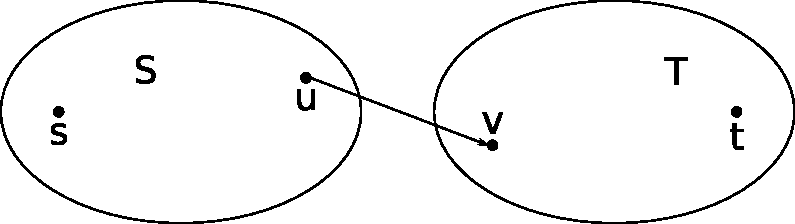
\includegraphics[scale=.5]{kap4SchnittWeg}
    \caption{Alle Kanten von $S$ nach $T$ entsprechen den Kapazitäten, die dem Fluss zur Verfügung stehen. Kein Fluss kann daher größer sein, als es der minimale Schnitt ist. Für alle $u \in S$ und alle $v \in T$ gilt, dass die Kapazitäten von $(u,v)$ voll ausgenutzt sind, wenn es einen maximalen Fluss gibt.}
    \label{kap4SchnittWeg}
  \end{figure}
  
  Aus \ref{kap4SatzMaxFMinS:augWeg} folgt \ref{kap4SatzMaxFMinS:minS}: Es gibt keine augmentierenden Wege, das heißt es gibt keinen Weg von $s$ nach $t$ im Restnetz. Sei $S := \{ s \} \cup \{v \in V \mid \text{ in } G_f \text{ gibt es einen Weg von $s$ nach $v$}\}$ und $T := V \setminus S$. Dann muss $s \in S$ und $t \in T$ gelten. $S, T$ ist dann ein Schnitt. Für alle $u \in S$ und $v \in T$ gilt $c(u,v) = f(u,v)$. Aus Abbildung \vref{kap4SchnittWeg} und Lemma \ref{Lemma42} folgt
  \[ |f| = f(S,T) = c(S,T) \]
  
      
  Aus \ref{kap4SatzMaxFMinS:minS} folgt \ref{kap4SatzMaxFMinS:fMax} ergibt sich aus obigen Korollar. $|f| \le c(S,T)$ gilt für alle Schnitte und alle Flüsse. Für den vorher definierten Schnitt muss $c(S,T)$ minimal sein. Aus $|f| = c(S,T)$ folgt, dass $c(S,T)$ minimal und $|f|$ maximal sein muss, $f$ also der maximale Fluss ist.
\end{Bew}

Aus \ref{kap4SatzMaxFMinS:augWeg} folgt die Korrektheit des Algorithmus von Ford"=Fulkerson. Aus \ref{kap4SatzMaxFMinS:minS} folgt dass der minimale Schnitt dem maximalen Fluss entspricht.

Betrachten wir noch einmal unser Beispiel aus Abbildung \vref{kap4Fluesse1}. Ein Minimaler Schnitt ist zum Beispiel $T = \{ v_2, t \}$ und $S = V \setminus T$. Dieser Schnitt hat eine Größe von $23$, also gilt für dieses Netz $|f^*| = 23$. Abbildung \vref{kap4Fluesse5} zeigt das Netzwerk und den Schnitt.

\begin{figure}[htb]
  \centering
  \includegraphics[scale=.75]{kap4Fluesse5}
  \caption{Die gestrichelte blaue Linie zeigt einen minimalen Schnitt der Größe $23$.}
  \label{kap4Fluesse5}
\end{figure}

\subsection{Edmonds"=Karp"=Algorithmus}
Im Algorithmus von Ford"=Fulkerson heißt es, dass ein augmentierender Weg gefunden werden soll. Wie dieser Weg gefunden werden soll ist nicht angegeben. Der Edmonds"=Karp"=Algorithmus ist eine Variante des Ford"=Fulkerson"=Algorithmus. Der augmentierende Weg wird dabei durch Breitensuche im Restnetz $G_f$ gefunden. Der so gefundene augmentierende Weg ist der kürzeste bezüglich der Anzahl der Kanten.

Die Laufzeit des Edmonds"=Karp"=Algorithmus zu bestimmen ist nicht ganz einfach. Sei $\delta_f(u,v)$ der Abstand (die Anzahl der Kanten des kürzesten Weges) zwischen $u,v \in V$ im Restnetz $G_f$. Dann gilt:
\begin{Lma}
  \hspace{\parindent}Beim Edmonds"=Karp"=Algorithmus gilt für alle Knoten $v \in V \setminus \{ s,t \}$: In jedem augmentierenden Schritt wächst der Abstand von $\delta_{f}(s,v)$ monoton.
\end{Lma}

\begin{Bem}
  \hspace{\parindent}$\delta_{f}(u,v)$ zählt die Kanten zwischen zwei Knoten im Restnetz $G_f$. Das heißt, wenn $\delta_{f}(u,v)$ sich ändert, muss mindestens eine Kante im Restnetz hinzugefügt oder entfernt worden sein. % Eine Kante im Restnetz wird nur unter bestimmten Änderungen des Flusses entfernt oder hinzugefügt (Nutzung einer zuvor ungenutzten Kante durch den Fluss, erhöhen des Flusses auf einer Kante bis zu ihrer vollen Kapazität, entfernen einer Kante aus dem Fluss, absenken des Flusses auf einer voll ausgelasteten Kante).% Eine Kante wird zum Restnetz hinzugefügt, wenn der Fluss auf einer komplett ausgelasteten Kante des Netzwerks abnimmt oder eine noch nicht genutzte Kante des Netzwerks in den Fluss einbezogen wird. Eine Kante wird aus dem Restnetz entfernt, wenn ihr Pendant im Netzwerk aus dem Fluss entfernt wird oder die durch den Fluss genutzte Kapazität einer Kante im Netzwerk auf die volle Kapazität der Kante ansteigt. % Wächst der Abstand im Restnetz zwischen $s$ und einem Knoten $v$ monoton, bedeutet das, dass die Anzahl der durch 
\end{Bem}

\begin{Bew}
  \hspace{\parindent} Das Lemma beweisen wir, in dem wir einen Beweis durch Widerspruch führen. $f$ bezeichne den Fluss vor einem Augmentierungsschritt, $f'$ den Fluss nach einem Augmentierungsschritt. Angenommen das Lemma gelte nicht und es existiere ein Augmentierungsschritt bei dem für mindestens einen Knoten $v$ $\delta_{f'}(s,v) < \delta_{f}(s,v)$ gelte. Unter allen Knoten, für die das gilt, wählen wir o.B.d.A. den Knoten als $v$, bei dem $\delta_{f'}(s,v)$ minimal sei. Gilt für einen Knoten $u$ $\delta_{f'}(s,u) < \delta_{f'}(s,v)$, so muss auch $\delta_f(s,u) \le \delta_{f'}(s,u)$ gelten, denn sonst hätten wir $u$ an Stelle von $v$ ausgewählt.
  
  $p' \leadsto u \to v$ sei der kürzeste Weg von $s$ nach $v$ in $G_{f'}$. $u$ ist also der direkte Vorgänge von $v$ auf diesem Weg. Das heißt $\delta_{f'}(s, u) < \delta_{f'}(s,v)$, also gilt $\delta_{f}(s,u) \le \delta_{f'} (s,u)$ (sonst hätten wir $u$ an Stelle von $v$ gewählt). Für die Kante $(u,v)$ gibt es im Fluss $f$ dann zwei Möglichkeiten: Entweder es gilt $f(u,v) < c(u,v)$ oder es gilt $f(u,v) = c(u, v)$.
  
  Falls $f(u,v) < c(u,v)$ folgt daraus, dass $(u,v)$ als Kante im Restnetz $G_f$ enthalten ist, der kürzeste Weg von $s$ nach $G_f$ also auf keinen Fall länger sein kann, als der Weg von $s$ nach $u$ und von dort nach $v$. Also $\delta_{f}(s,v) \le \delta_{f}(s,u) + 1$ ($+1$ für die Kante $u \to v$). Dann gilt $\delta_{f}(s, u) + 1 \le \delta_{f'}(s,u) +1 = \delta_{f'}(s,v)$. Daraus folgt aber $\delta_{f}(s,v) \le \delta_{f'}(s,v)$, was unsere Annahme zum Widerspruch führt!
  
  Betrachten wir den Fall $f(u,v) = c(u,v)$. In diesem Fall ist $(u,v)$ keine Kante in $G_f$, aber eine Kante in $G_{f'}$, das heißt der augmentierende Weg $p$ muss die Kante $(v,u)$ enthalten. Der Edomnds"=Karp"=Algorithmus erweitert den Fluss immer nur entlang kürzester Wege, $p$ muss also der kürzeste Weg von $s$ nach $t$ im Restnetz $G_{f}$ sein, also ist $(v, u)$ Teil des kürzesten Wegs von $s$ nach $u$. Also
    \begin{align*}
      \delta_f(s,v) &= \delta_f(s,u) - 1 \\
                    &\le \delta_{f'}(s,u) -1 \\
                    &= \delta_{f'}(s,v) -2\\
                    &< \delta_{f'}(s,v)
    \end{align*}
    $\delta_f(s,v) < \delta_{f'}(s,v)$ ist ein Widerspruch zu unserer Annahme, das Lemma somit bewiesen.
\end{Bew}

Nachdem wir bewiesen haben, dass der Abstand zwischen einem Knoten $v$ (mit $v \neq s$ und $v \neq t$) und $s$ im Restnetz bei jedem Augmentierungsschritt monoton wächst, können wir uns die Laufzeit des Algorithmus näher anschauen.

%vorlesung 16 13.12.2010 (Mo)
\begin{Lma}
  \hspace{\parindent}Der Algorithmus von Edmonds"=Karp führt auf einem Netz mit $n = |V|$ Knoten und $m = |E|$ Kanten höchstens $\mathcal{O}(n \cdot m)$ Augmentierungen durch.
\end{Lma}
\begin{Bew}
  \hspace{\parindent}Eine Kante $(u,v)$ auf einem augmentierendem Weg $p$ wird \textit{kritisch} genannt genau dann, wenn $c_f(p) = c_f(u,v)$, wobei $c_f(p)$ die Kapazitätserhöhung ist und $c_f(u,v)$ die Restkapazität von $(u,v)$. Das heißt der Fluss wird um $c_f(u,v)$ erhöht. Nach der Augmentierung verschwindet die kritische Kante aus dem Restnetz, da ihre Kapazität dann ganz durch den Fluss genutzt wird. Bevor $(u,v)$ wieder im Restnetz erscheint, muss $(v,u)$ auf einem augmentierendem Weg liegen.
  
  Sei $f$ der Fluss bei dem $(u,v)$ kritisch war, auf dem nach dem Edmonds"=Karp"=Algorithmus gewählten augmentierenden Weg, also dem kürzesten Weg von $s$ nach $t$ im Restnetz $G_f$. Dann gilt $\delta_f(s,v) = \delta_f(s,u) + 1$, da die Kante $(u,v)$ nur dann als kritisch bezeichnet werden kann, wenn sie auf dem augmentierenden Weg liegt und $v$ auf $u$ folgt. Sei $f'$ der Fluss bei dem $(v,u)$ auf dem augmentierenden Weg liegt, nachdem $(u,v)$ in einer vorhergehenden Augmentierung kritisch war ($(u,v)$ war im Restnetz vom Vorgänger von $f'$ also nicht enthalten). Nach obigen Lemma wächst $\delta_f(s,v)$ monoton. Daher gilt

  \begin{align*}
    \delta_{f'}(s, u) &= \delta_{f'}(s,v)+1\\
                      &\ge \delta_f(s,v) + 1\\
                      &= \delta_f(s,u) + 2
  \end{align*}
  
  Das heißt wenn $(u,v)$ zwei Mal kritisch sein soll, erhöht sich der Abstand derweil im Restnetz um mindestens 2. Er kann höchstens $n-2$ werden, also kann eine Kante höchstens $\frac{n-2}{2} = \mathcal{O}(n)$ oft kritisch werden. Da das für jede Kante gilt, gibt es höchstens $\mathcal{O}(n \cdot m)$ Augmentierungen.
\end{Bew}

Der Edmonds"=Karp"=Algorithmus führt pro Augmentierung drei Schritte durch. Er sucht nach einem Weg von $s$ nach $t$ im Restnetz $G_f$ per Breitensuche, er erhöht den Fluss entlang dieses Wegs und er aktualisiert das Restnetz $G_f$. Es sollte offensichtlich sein, dass die letzten beiden Schritte in $\mathcal{O}(m)$ liegen. Die Breitensuche braucht normalerweise $\mathcal{O}(m+n)$ Zeit, $\mathcal{O}(n)$ für die Initialisierung und $\mathcal{O}(m)$ für das Prüfen der Adjazenzlisten. Wir halten das Restnetz lediglich für das Finden des Weges von $s$ nach $t$ vor und aktualisieren es in einem eigenen Schritt. Daher können wir hier auch für die Breitensuche eine Laufzeit von $\mathcal{O}(m)$ veranschlagen.

Da der Edmonds"=Karp"=Algorithmus maximal $\mathcal{O}(n \cdot m)$ Augmentierungen mit einer Laufzeit von jeweils $\mathcal{O}(m)$ durchführt ergibt sich folgender Satz:

\begin{Satz}
  \hspace{\parindent}Der Algorithmus von Edmonds"=Karop hat eine Gesamtlaufzeit von $\mathcal{O}(n \cdot m^2)$. Das liegt in $\mathcal{O}(n^5)$, weil wir $\mathcal{O}(m)$ mit  $\mathcal{O}(n^2)$ abschätzen können.
\end{Satz}

Das finden maximaler Flüsse ist intensiv erforscht worden. Ford und Fulkerson stellten den ersten Algorithmus dazu vor, Edmonds und Karp den ersten, der in polynomieller Zeit arbeitet. Seitdem sind etliche Verbesserungen erzielt und neue Algorithmen gefunden worden:
\begin{itemize}
  \item Goldberg stellte einen Algorithmus vor, der in $\mathcal{O}(n^2 \cdot m) = \mathcal{O}(n^4)$ arbeitet.
  \item 1986 stellten Goldberg und Tarjan einen Algorithmus mit einer Laufzeit von $\mathcal{O}(n \cdot m \cdot \log{\frac{n^2}{m}})$ vor.
  \item Mehlhorn, Cheryan, Hagerup veröffentlichten 1997 einen Algorithmus, der in $\mathcal{O}(n \cdot m + n^2 \log n)$ den maximalen Fluss eines Netzwerks findet.
\end{itemize}

Der Algorithmus von Edmonds"=Karp hat den Vorteil, dass er einfach nutzbar ist, auch wenn $\mathcal{O}(n^5)$ eine relativ große Laufzeit ist. $\mathcal{O}(n^5)$ ist dennoch polynomiell und nicht exponentiell.

\section{Bipartites Matching}
\begin{Def}[Matching (Paarung)]
  \hspace{\parindent}Sei $G=(V,E)$ ein ungerichteter Graph. Ein \textit{Matching} ist eine Teilmenge $M \subset E$, so dass keine zwei Kanten in $M$ einen Endpunkt gemeinsam haben.
\end{Def}

\begin{Def} [maximales Matching (maximal matching)]
  \hspace{\parindent}Ein Matching $M$, das nicht mehr erweitert werden kann, nennt man \textit{maximales Matching}. Das heißt es existiert kein Matching $M'$, so dass $M \subsetneq M'$.
\end{Def}

\begin{Def}[größtes Matching (maximum matching)]
  \hspace{\parindent}$M$ sei ein Matching. Gilt $|M| \ge |M'|$ für alle Matchings $M'$, so nennt man $M$ \textit{größtes Matching}.
\end{Def}

\begin{figure}[htb]
  \centering
  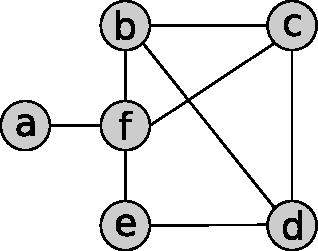
\includegraphics[scale=.66]{kap4MatchingBsp}
  \caption{Im gezeigten Graphen bildet $\{(b,d), (c,f)\}$ ein maximales aber kein größtes Matching. Größtes Matching ist $\{(a,f),(e,d),(b,c)\}$.}
  \label{kap4MatchingBsp}
\end{figure}

Jedes größte Matching ist maximal, aber nicht jedes maximale Matching ist größtes Matching. Ein maximales Matching ist leicht zu finden: man fügt "`greedy"' Kanten zu einer Menge hinzu, bis das Matching durch keine der verbliebenen Kanten erweitert werden kann. Ein größtes Matching lässt sich durch einen Netzwerk"=Fluss finden.

\begin{Def}[Bipatiter Graph]
  \hspace{\parindent}Ein Graph $G=(V,E)$ heißt bipartit (Paar) genau dann, wenn eine Partition $V = V_1 \cupdot V_2$ existiert, so dass alle Kanten einen Endpunkt in $V_1$ und einen in $V_2$ haben.
\end{Def}

\begin{figure}[htb]
  \centering
  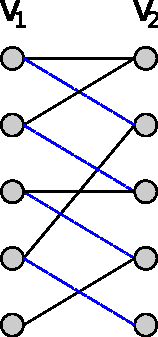
\includegraphics[scale=.75]{kap4BipartitesMatching1}
  \caption{Zu sehen ist ein bipartiter Graph. Die blauen gestrichelten Kanten bilden ein Matching.}
  \label{kap4BipartitesMatching1}
\end{figure}

Die Suche nach einem größten Matching in einem bipartiten Graphen lässt sich auf das Flussproblem zurückführen. Dazu schaffen wir zwei zusätzliche Knoten: eine Quelle $s$ und eine Senke $t$. Wir fügen nun gerichtete Kanten $(s,v)$ für alle Knoten $v \in V_1$ und gerichtete Kanten $(u,t)$ für alle Knoten $u \in V_2$ ein und gewichten alle Kanten mit Kapazität $1$. Auch die Kanten, die im bipartiten Graphen enthalten waren gewichten wir mit Kapazität $1$ und wandeln sie zu gerichteten Kanten, die von Knoten aus $V_1$ zu Knoten aus $V_2$ verlaufen.

\begin{figure}[htb]
  \centering
  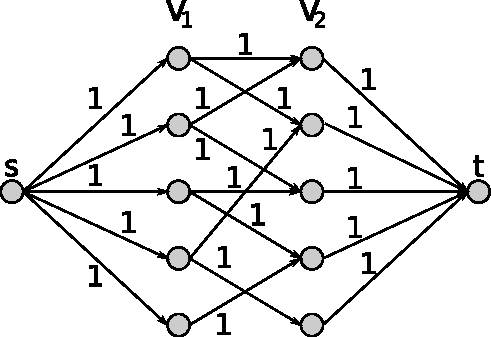
\includegraphics[scale=.8]{kap4BipartitesMatching2}
  \caption{Der bipartite Graph aus Abbildung \vref{kap4BipartitesMatching1} wurde zu einem Netzwerk erweitert.}
  \label{kap4BipartitesMatching2}
\end{figure}


Anschließend bestimmen wir den maximalen Fluss in dem entstandenen Netzwerk, zum Beispiel mit dem Edmonds"=Karp"=Algorithmus. Das größte Matching besteht dann aus den Kanten, die im Fluss mit Kapazität $1$ enthalten sind und von $V_1$ nach $V_2$ führen.

\begin{figure}[htb]
  \centering
  \includegraphics[scale=.8]{kap4BipartitesMatching3}
  \caption{Im Netzwerk aus Abbildung \vref{kap4BipartitesMatching2} wurde der dargestellte Fluss (blaue gestrichelte Kanten) gefunden. Die von $V_1$ nach $V_2$ verlaufenden Kanten des Flusses bilden ein maximales Matching.}
  \label{kap4BipartitesMatching3}
\end{figure}

Gibt es in einem Netz nur ganzzahlige Kapazitäten, so folgt daraus, dass es auch einen ganzzahligen maximalen Fluss gibt, welcher vom Ford"=Fulkerson"=Algorithmus beziehungsweise einer Variante davon, wie zum Beispiel dem Edmonds"=Karp"=Algorithmus, gefunden wird. Beide Algorithmen führen lediglich Addition und Subtraktion aus, die Kapazitäten bleiben also immer ganzzahlig. Bei dem von uns erzeugten Netzwerk können die Kanten durch den Fluss also immer nur mit einer Kapaztität von $0$ oder $1$ genutzt werden. Um die Korrektheit unseres Vorgehens nachzuweisen müssen wir also lediglich zeigen, dass der maximale Fluss in einem zum Netzwerk erweiterten bipartitem Graphen wirklich einem größten Matching entspricht, also $|f^*| = |M|$ wobei $f^*$ maximaler Fluss in $G'$ ist und $M$ größtes Matching in $G$.

Sei $M$ größtes Matching in $G$, dann lässt sich ein Fluss der Größe $|M|$ konstruieren. Im zum Netzwerk erweiterten Graphen $G'$ folgen wir dazu den Kanten von $s$ zu allen Knoten aus $V_1$, die Teil des Matchings sind. Von diesen Knoten aus folgen wir den im Matching enthaltenen Kanten nach $V_2$ und dort den Kanten zu $t$. Das heißt ein Maximaler Fluss muss so groß sein, wie das größte Matching.

Sei $f^*$ maximaler Fluss. Rufen wir uns kurz in Erinnerung, wie wir $G'$ erzeugt haben: alle Kanten verlaufen von $s$ zu Knoten aus $V_1$, von dort zu Knoten aus $V_2$ und von dort nach $t$. Jede Kante hat eine Kapazität von $1$. Daraus folgt, dass alle Kanten in $f^*$ eine Kapazität von $0$ oder $1$ haben müssen und $f^*$ ganzzahlig sein muss. Zwei Kanten, die der Fluss mit Kapazität $1$ nutzt und die zwischen $V_1$ und $V_2$ verlaufen können weder den selben Anfangs-, noch den selben Endknoten haben. In jeden Knoten aus $V_1$ (die Anfangsknoten einer solchen Kante) fließt nur eine Kante mit Kapazität $1$. Aus jedem Knoten von $V_2$ (Endknoten der betrachteten Kante) führt nur eine Kante auch mit einer Kapazität von $1$. Daraus folgt, dass alle Kanten des Flusses, die zwischen $V_1$ und $V_2$ verlaufen ein Matching $M$ bilden mit $|M| = |f^*|$.

% Wir haben also gesehen, dass es einen Fluss geben muss, der mindestens so groß sein muss, wie jedes Matching. Wir haben auch gesehen, dass es zu jedem Fluss ein Matching geben muss. $\{s\} \cup V_1, \{t\} \cup V_2$ ist ein Schnitt im Netzwerk. Wir wissen, dass ein Fluss nicht größer sein kann, als ein Schnitt. Da es keine direkten Kanten von $s$ nach $t$ gibt, ist der Fluss genau so groß, wie die von ihm genutzten Kapazitäten zwischen $V_1$ und $V_2$. Jede Kante hat eine Kapazität von maximal $1$. $f(V_1, V_2)$ entspricht also der Anzahl der genutzten Kanten. Daraus folgt $|M| \le |f^*| \le |M|$, also $|M| = |f^*|$.

Betrachten wir abschließend die Laufzeit zum Finden des Matchings. Der Algorithmus von Ford und Fulkerson braucht $\mathcal{O}(|f^*| \cdot m)$ Zeit zum Finden des maximalen Flusses, aus dem sich direkt das Matching ergibt. Den maximalen Fluss in einem Netzwerk, das aus einem bipartiten Graphen hervorgegangen ist, können wir leicht abschätzen: $|f^*| \le \frac{n}{2}$. Ein größtes Matching in einem bipartiten Graphen $G = (V, E)$ kann also in in $\mathcal{O}(n \cdot m)$ gefunden werden.

%Edmonds"=Karp funktioniert auch in Netzwerken mit nichtganzzahligen Kapazitäten. Folgt irgendwie aus Laufzeitanalyse, so ich es richtig verstanden habe....
